\documentclass{article}
\usepackage{pgfplots}
\title{KEEL: ROC output}
\begin{document}
\maketitle
\hfill \break
File: TEST
\hfill \break
\hfill \break
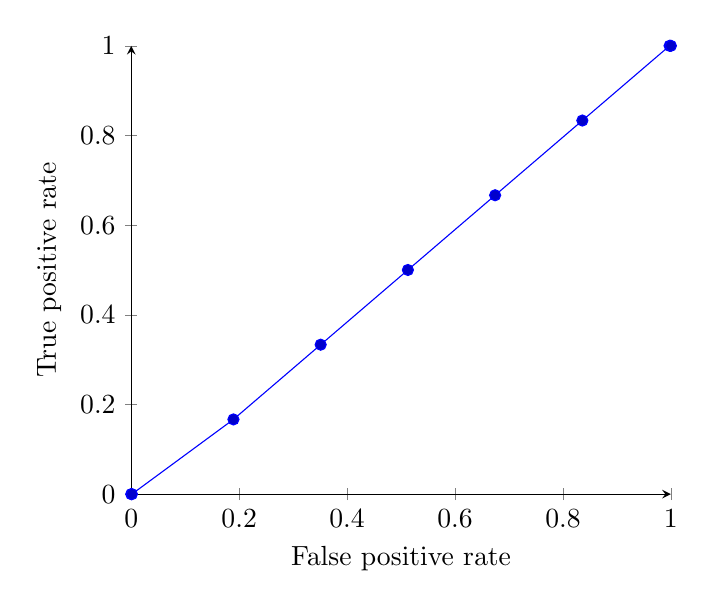
\begin{tikzpicture}
\begin{axis} [xlabel=False positive rate,
ylabel=True positive rate,axis x line=bottom,
axis y line=left]
\addplot coordinates { (0,0)(0.0012062726176115801,0.0)(0.18938480096501822,0.16666666666666666)(0.3510253317249701,0.3333333333333333)(0.5126658624849214,0.5)(0.6743063932448659,0.6666666666666666)(0.8359469240048103,0.8333333333333333)(0.9975874547647547,0.9999999999999999) (1,1) };\end{axis}
\end{tikzpicture}\hfill \break
 AUC:0.4077201447526993
\hfill \break
\hfill \break
File: TRAINING
\hfill \break
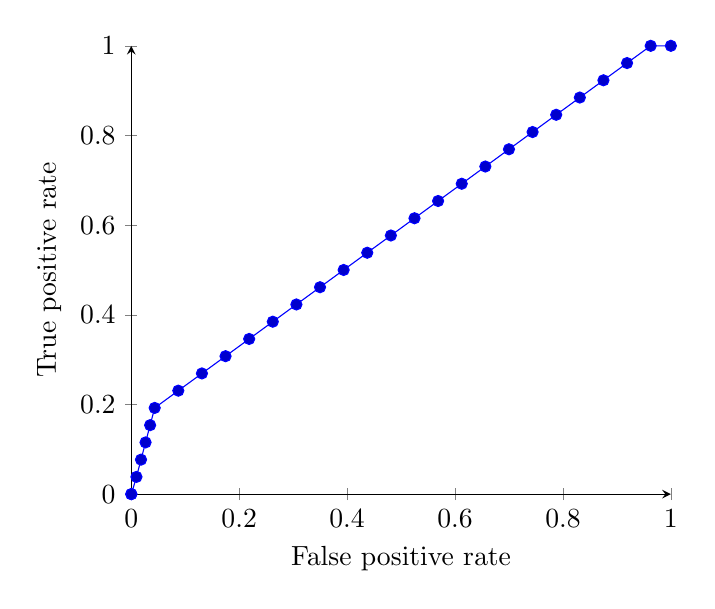
\begin{tikzpicture}
\begin{axis} [xlabel=False positive rate,
ylabel=True positive rate,axis x line=bottom,
axis y line=left]
\addplot coordinates { (0,0)(3.0184123151222455E-4,0.0)(0.009658919408391193,0.038461538461538464)(0.018110473890733475,0.07692307692307693)(0.026562028373075725,0.11538461538461539)(0.035013582855417974,0.15384615384615385)(0.043465137337760223,0.19230769230769232)(0.08723211590703259,0.23076923076923078)(0.13099909447630495,0.2692307692307693)(0.1747660730455773,0.3076923076923077)(0.21853305161484968,0.34615384615384615)(0.26230003018412207,0.3846153846153846)(0.30606700875339443,0.423076923076923)(0.3498339873226668,0.46153846153846145)(0.39360096589193916,0.4999999999999999)(0.4373679444612115,0.5384615384615383)(0.4811349230304839,0.5769230769230768)(0.5249019015997562,0.6153846153846152)(0.5686688801690286,0.6538461538461536)(0.612435858738301,0.6923076923076921)(0.6562028373075733,0.7307692307692305)(0.6999698158768457,0.7692307692307689)(0.7437367944461181,0.8076923076923074)(0.7875037730153904,0.8461538461538458)(0.8312707515846628,0.8846153846153842)(0.8750377301539352,0.9230769230769227)(0.9188047087232075,0.9615384615384611)(0.9625716872924799,0.9999999999999996) (1,1) };\end{axis}
\end{tikzpicture}\hfill \break
 AUC:0.5712345306368852
\hfill \break
\end{document}